	\section{Experimentos}
	Neste capítulo apresenta a descrição, o resultado e a análise do experimento realizado.
	
	Objetivo é verifica a eficácia do RAID5 em relação à RAID0 e RAID1.
	
	A comparação será feita pela execução das operações de leitura ou escrita, utilizando arquivos de quatro tamanhos diferentes de 1KB, 100KB, 1MB e 10MB.
	
	Serão realizado dois tipos de experimentos.
	\subsubsection{Teste de latência}
	Focaliza em medir a diferença de tempo que demora para executar certa quantidade das operações entre os três tipos de RAID.
	Somente um cliente solicita 1000 operações de leitura ou escrita para servidor e mede quanto tempo o sistema demora para concluir todas as solicitações.
	
	\subsubsection{Teste de vazão}	
	Focaliza em medir a diferença da quantidade de operações executadas em certo intervalo de tempo entre os três tipos de RAID.
	
	\subsection{Resultaos}
	
	\subsubsection{Teste de latência}
	
	A Figura~\ref{fig:lat_leit} mostra o gráfico de resultado para leitura dos arquivos. 
	No gráfico percebe-se que o RAID1 tem menor latência.
	
	Mas conforme aumentando o tamanho do arquivo as latências dos três RAID tendem a ter mesmos valores.
	
	
	
	%Como neste sistema a transmissão de dados entre cliente e servidor de armazenamento não está implementa do em \textit{multithread}
	\begin{figure}[htb]
		\begin{center}
			
			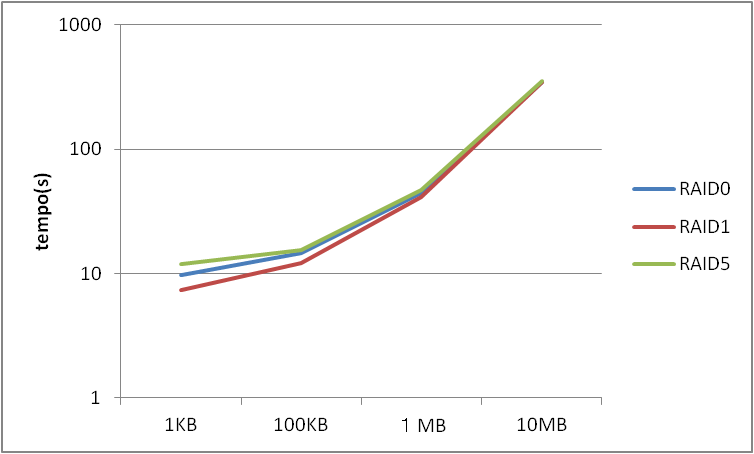
\includegraphics[clip,width=10.0cm]{images/resultados/latencia_leitura.png}
			\caption{Gráfico de leitura para teste de latência}
			\label{fig:lat_leit}
		\end{center}
	\end{figure}
	
	A Figura~\ref{fig:lat_esc} mostra o gráfico de resultado para escrita dos arquivo para cada tipo de RAID.
	
	\begin{figure}[htb]
		\begin{center}
			
			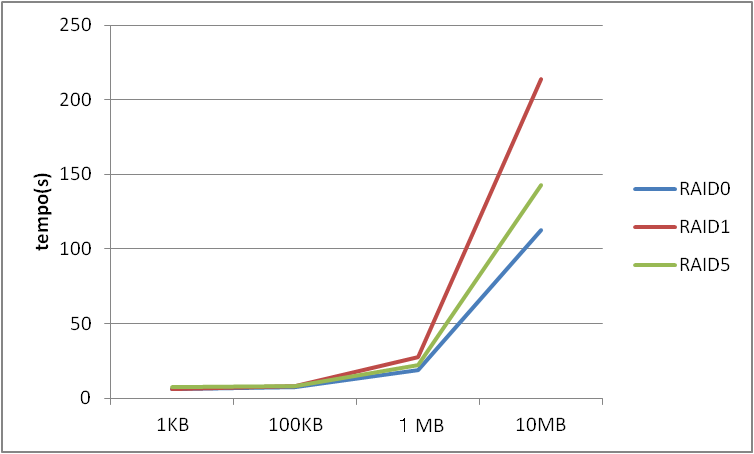
\includegraphics[clip,width=10.0cm]{images/resultados/latencia_escrita.png}
			\caption{Gráfico de escrita para teste de latência}
			\label{fig:lat_esc}
		\end{center}
	\end{figure}
	
	\subsubsection{Teste de vazão}	
	
	\section{Conclusões do Capítulo}